\documentclass{standalone}
\usepackage{pgfplots}
\pgfplotsset{compat=1.18}

\begin{document}

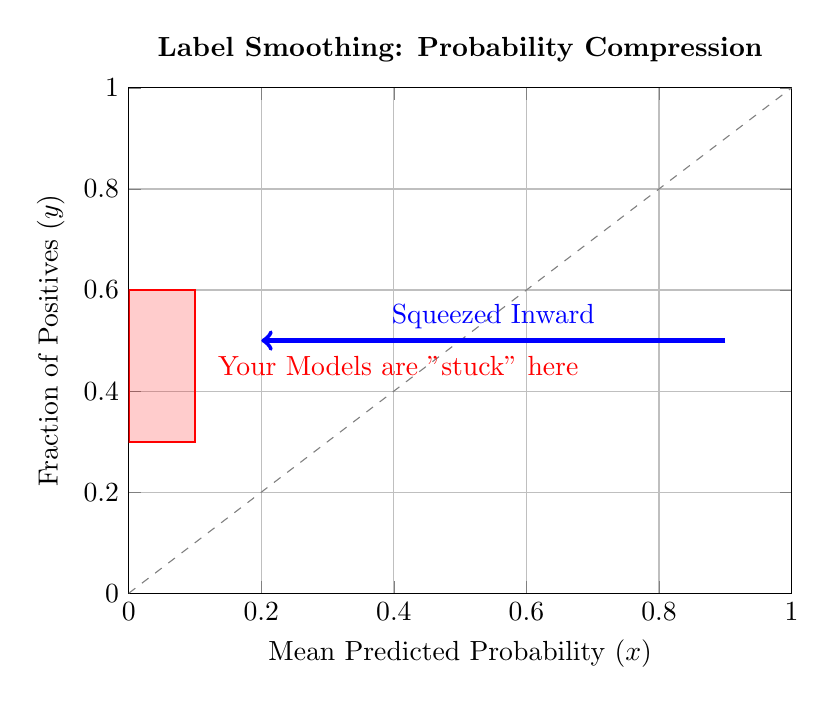
\begin{tikzpicture}
\begin{axis}[
    title={\textbf{Label Smoothing: Probability Compression}},
    xlabel={Mean Predicted Probability ($x$)},
    ylabel={Fraction of Positives ($y$)},
    xmin=0, xmax=1,
    ymin=0, ymax=1,
    grid=both,
    width=10cm, height=8cm
]
    % Perfectly Calibrated Line
    \addplot [gray, dashed] coordinates {(0,0)(1,1)};
    
    % The "Collapsed" Data Area
    \draw[red, thick, fill=red, fill opacity=0.2] (0,0.3) rectangle (0.1,0.6);
    \node[red, anchor=west] at (axis cs:0.12, 0.45) {Your Models are "stuck" here};
    
    % Arrow showing the "Squeeze"
    \draw[->, ultra thick, blue] (axis cs:0.9, 0.5) -- (axis cs:0.2, 0.5) 
        node[midway, above, text=blue] {Squeezed Inward};

\end{axis}
\end{tikzpicture}
\end{document}